\documentclass{homework}

\usepackage[table]{xcolor}
\usepackage{booktabs}
\usepackage{tikz}
\newcommand{\myname}{Kristof Nemeth}
\newcommand{\assignment}{Quiz 3}
\newcommand{\duedate}{}
\newcommand{\course}{Coding Theory}

\renewcommand{\C}{\mathcal{C}}
\setcounter{MaxMatrixCols}{29}

\begin{document}

Consider the field $\F = \F_{64}$
\begin{problem}
  The group $\F*$ is of order $63$. Therefore, the possible
  orders of elements in  $\F^*$ are $1,3,7,9,21$, and $63$

  There is of course, one element of order 1. There are $ \phi(3)=2$ elements of
  order 3, $\phi(7) = 6$ elements of order 7, $\phi(9) = 6$ elements of order
  $9$, $\phi(21) = 12$ elements of order 21, and $\phi(63) = 36$ primitive
  elements.

\end{problem}

\begin{problem}
  Let $\alpha$ be a primitive element of $\F$. Then the primitive elements in
  $\F^*$
  are:

  \[
    \begin{aligned}
      C_{\alpha^1} = &\{\alpha^1,\alpha^{2}, \alpha^{4}, \alpha^{8}, \alpha^{16},
      \alpha^{32}\}\\
      C_{\alpha^5} = &\{\alpha^5,\alpha^{10}, \alpha^{20}, \alpha^{40}, \alpha^{17},
      \alpha^{34}\}\\
      C_{\alpha^{11}} = &\{\alpha^{11},\alpha^{22}, \alpha^{44}, \alpha^{25}, \alpha^{50},
      \alpha^{37}\}\\
      C_{\alpha^{13}} = &\{\alpha^{13},\alpha^{26}, \alpha^{52}, \alpha^{41}, \alpha^{19},
      \alpha^{38}\}\\
      C_{\alpha^{23}} = &\{\alpha^{23},\alpha^{46}, \alpha^{29}, \alpha^{58}, \alpha^{53},
      \alpha^{43}\}\\
      C_{\alpha^{31}} = &\{\alpha^{31},\alpha^{62}, \alpha^{61}, \alpha^{59}, \alpha^{55},
      \alpha^{47}\}\\
    \end{aligned}
  \]

  The primitive elements above have already been arranged by the cyclotomic
  coset that they belong to. Hence this gives us the following primitive
  polynomials:

  \[
    \begin{aligned}
      M^{(1)}(x) &=
      (x-\alpha^{1})(x-\alpha^{2})(x-\alpha^{4})(x-\alpha^{8})(x-\alpha^{16})(x-\alpha^{32})\\
      M^{(5)}(x) &=
      (x-\alpha^{5})(x-\alpha^{10})(x-\alpha^{20})(x-\alpha^{40})(x-\alpha^{17})(x-\alpha^{34})\\
      M^{(11)}(x) &=
      (x-\alpha^{11})(x-\alpha^{22})(x-\alpha^{44})(x-\alpha^{25})(x-\alpha^{50})(x-\alpha^{37})\\
      M^{(13)}(x) &=
      (x-\alpha^{13})(x-\alpha^{26})(x-\alpha^{52})(x-\alpha^{41})(x-\alpha^{19})(x-\alpha^{38})\\
      M^{(23)}(x) &=
      (x-\alpha^{23})(x-\alpha^{46})(x-\alpha^{29})(x-\alpha^{58})(x-\alpha^{53})(x-\alpha^{43})\\
      M^{(31)}(x) &=
      (x-\alpha^{31})(x-\alpha^{62})(x-\alpha^{61})(x-\alpha^{59})(x-\alpha^{55})(x-\alpha^{47})
    \end{aligned}
  \]

\end{problem}

\begin{problem}
  On page 105, we can see that there are $9$ cyclotomic cosets of size $6$ for
  $\F^*$. This accounts for 54 elements, which is greater than the number of
  primitive elements. Simply put, while each primitive element has a minimal
  polynomial of degree 6 in $\F^*$, the converse is not necessarily true: not every
  polyomial of degree 6 will have primitive elements as their roots.
  The three cosets in question have represantatives $3,7 $ and $15$, all of
  which are not relatively prime to $63$. Hence, none of the elements in these
  three cosets are actually primitive. The remaining 6 cosets leaves us with
  $36$ elements, which is exactly the $36$ primitive elements in $\F^*$. The $54$
  elements which have cyclotomic cosets of size $6$ are those elements which are
  not contained in any proper subfields of $\F$
\end{problem}

\begin{problem}
  The subfields of $GF(2^6)$ are shown below.
  \begin{figure}[h!]
    \begin{center}
      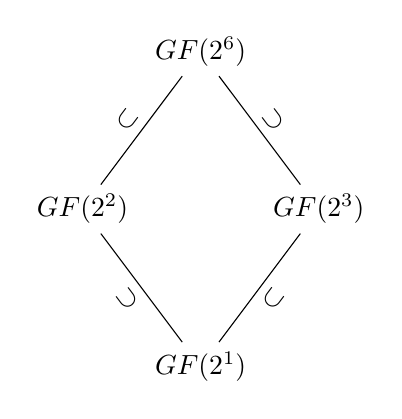
\begin{tikzpicture}[scale=1,auto]
        \node (F64) at (1.5,4) {$GF(2^6)$};
        \node (F4) at (0,2) {$GF(2^2)$};
        \node (F8) at (3,2) {$GF(2^3)$};
        \node (F2) at (1.5,0) {$GF(2^1)$};
        \path[-]
          (F64) edge node[midway,sloped,anchor=south] {$\subset$} (F4)
          (F64) edge node[midway,sloped,anchor=south] {$\supset$} (F8)
          (F4) edge node[midway,sloped,anchor=north] {$\supset$} (F2)
          (F8) edge node[midway,sloped,anchor=north] {$\subset$} (F2)
          ;
      \end{tikzpicture}
    \end{center}
    \caption{Subfields of $GF(2^6)$}
    \label{fig:}
  \end{figure}

\end{problem}

\end{document}
